\documentclass[12pt]{gatechthesis}  
\usepackage{url} 
\usepackage{listings}
\usepackage{float}
\usepackage{xcolor}

\hypersetup{urlcolor=cyan}


\definecolor{codegreen}{rgb}{0,0.6,0}
\definecolor{codegray}{rgb}{0.5,0.5,0.5}
\definecolor{codepurple}{rgb}{0.58,0,0.82}
\definecolor{backcolour}{rgb}{0.95,0.95,0.92}

\lstdefinestyle{mystyle}{
    backgroundcolor=\color{backcolour},   
    commentstyle=\color{codegreen},
    keywordstyle=\color{magenta},
    numberstyle=\tiny\color{codegray},
    stringstyle=\color{codepurple},
    basicstyle=\ttfamily\footnotesize,
    breakatwhitespace=false,         
    breaklines=true,                 
    captionpos=b,                    
    keepspaces=true,                 
    numbers=left,                    
    numbersep=5pt,                  
    showspaces=false,                
    showstringspaces=false,
    showtabs=false,                  
    tabsize=2
}

\lstset{style=mystyle}

% preamble

\title{Towards integrating io\_uring into the Haskell GHC Runtime}
\author{Tsz Hang Kiang}
\approvaldate{August 2nd, 2023}
\school{School of Computer Science}
\bibliography{references}

% document body
\begin{document}

\makeTitlePage{Aug}{2023}
 % In \begin{approvalPage}{N}, the parameter N is the number of members in the committee. If this is less than 4, the layout of the page is single-column rather than two-column, so change the value accordingly.

\begin{approvalPage}{4}

% Add people in the following format:
% \committeeMember{Member Name}{Member Department/Position}{Member Affiliation}

\committeeMember{Dr. Vivek Sarkar}{School of Computer Science}{Georgia Institute of
Technology}
\committeeMember{Dr. Akihiro Hayashi}{School of Computer Science}{Georgia Institute of Technology}
% \committeeMember{Dr. Raymond Palmer}{Department of Physics}{Ivy University}
% \committeeMember{Dr. Kimiyo Hoshi}{Division of Science}{Astronomy College of Tokyo}
% \committeeMember{Dr. Michael Holt}{Department of Physics}{Georgia Institute of Technology}
\\ % <- add space for alignment, if necessary
% \committeeMember{Dr. Kent Nelson}{Medical Sciences}{Georgia Institute of Technology}

\end{approvalPage}

\begin{frontmatter}
    % \input{acknowledgments}
    \makeTOC
    % \makeListOfTables
    \makeListOfFigures
    % \input{abbrevs}
    \begin{abstrct}

With the recent introduction of the new Linux \texttt{io\_uring} subsystem for
asynchronous system calls, we explore both the performance and design
considerations of integrating \texttt{io\_uring} into the Glasgow Haskell Compiler (GHC)
runtime. We draw inspiration from the existing Multicore IO (MIO)
\texttt{EventManager} \cite{mio}, a highly refined and tested polling-based
(e.g. \texttt{epoll}, \texttt{kqueue}, \texttt{select}) approach
to non-blocking I/O,
to create \newline
\texttt{URingManager}, our approach to utilizing \texttt{io\_uring}
in the runtime. We find that in networking workloads, using
\texttt{URingManager},
\texttt{io\_uring}-driven asynchronous I/O is capable of achieving performance
equivalent to that of the MIO \texttt{EventManager} with epoll. In terms of
design, we find that our \texttt{URingManager} is also able to benefit from
the cleaner asynchronous interface that \texttt{io\_uring} provides when
compared to Linux Asynchronous I/O (AIO) and polling methods.

\end{abstrct}

\end{frontmatter} 

\begin{thesisbody}
    \chapter{Introduction}

Currently, a popular and well-tested approach to efficient asynchronous I/O is through the
use of polling mechanisms. Depending on the operating system, system calls such as \texttt{epoll}, \texttt{kqueue}, or \texttt{select},
can be used to register a file descriptor for interest in potentially blocking I/O,
as well as receive notification that the file descriptor is ready and guaranteed to not
block on the desired I/O operation. This design has also been the basis of concurrent Haskell
programs.
The design was refined upon, into what is now the MIO \texttt{EventManager}
\cite{mio, scalableIO},
where now multiple cores could each manage their own pending I/O notifications, and schedule their respective threads.

More recently, Linux introduced \texttt{io\_uring}, a new asynchronous system call facility that uses a
completion-based paradigm, fundamentally different from the readiness-based paradigm of polling mechanisms.
In \texttt{io\_uring}, instead of waiting for the kernel to notify user threads of readiness events as in epoll,
a task carrying a request to perform a potentially blocking I/O operation is sent to the kernel,
and when the operation is complete, the kernel responds with the result. Theoretically,
the design is expected to be more efficient
due to fewer syscalls required. However, in practice, the possible
performance gains have come into question.

Hence, our motivation for writing \texttt{URingManager}: firstly trying to gauge the performance of \texttt{io\_uring},
especially with Haskell’s lightweight green threading-based runtime system, and secondly,
exploring this new paradigm of asynchronous programming.

    \chapter{Background}

\section{The MIO and the GHC Runtime}
Haskell programs use a green threading model for concurrency. The GHC runtime system (RTS) is
responsible for the scheduling of these lightweight Haskell threads. Both a single-core “unthreaded”
version and a multicore version \cite{multicoreSupport} of the RTS are available. We will focus on only the multicore
version of the RTS for the remainder of this paper.

In the RTS, a Capability is a virtual CPU for executing Haskell code, the number of which are in the
runtime chosen by the user \cite{multicoreSupport}. Haskell threads are then assigned to these Capabilities to be 
executed. Haskell threads come in three flavors with respect to Capabilities: unbounded, bounded
to a Capability, bounded to an operating system thread. These threads are created with the functions
\texttt{forkIO}, \texttt{forkOn}, and \texttt{forkOS} respectively. 

The definition of the MIO \texttt{EventManager} and notable related
functions are shown in Figure \ref{fig:EventManager}. 

% TODO: Force this to be closer to the text?
\begin{figure}[ht]
  \centering
  \lstinputlisting[language=Haskell]{figures/code/EventManager.hs}
  \caption[\texttt{EventManager} definition and related functions]{
  Definition for \texttt{EventManager} and related functions} 
  \label{fig:EventManager}
\end{figure}


In the definition, \texttt{emBackend} holds an existentially quantified Backend value, allowing for abstraction over
different \texttt{EventManager} Backend implementations, such as \texttt{epoll}-based or \texttt{kqueue}-based. Also of interest is \texttt{emFds},
an array-backed mapping of file descriptors to callbacks, which stores metadata for currently registered requests.

To understand the type signature of the \texttt{registerFd}, specifically how the IO callback is used to wake up a thread,
we need a short detour to explain the Concurrent Haskell \texttt{MVar} synchronization primitive \cite{concurrentHaskell}.
The \texttt{MVar} has the following primitive operations shown in Figure \ref{fig:MVar}. An \texttt{MVar a} can either hold a value of type \texttt{a}, or be empty.

\begin{figure}[H]
  \centering
  \lstinputlisting[language=Haskell]{figures/code/MVar.hs}
  \caption[\texttt{MVar} Functions]{
    \texttt{MVar} Functions
  }
  \label{fig:MVar}
\end{figure}


If \texttt{takeMVar} is called on an empty \texttt{MVar}, the calling Haskell thread will block until another thread calls \texttt{putMVar}
to put a value inside the \texttt{MVar}. Upon successfully taking the \texttt{MVar},
the \texttt{MVar} will become empty.
This Haskell thread blocking is efficient because under the hood,
the \texttt{MVar} is tracked by the RTS, and the thread will sleep until woken up when the RTS realizes the \texttt{MVar} is non-empty.

Thus, the callback passed into \texttt{registerFd} is a \texttt{putMVar} operation is an empty \texttt{MVar}
 Upon calling \texttt{registerFd}, the \texttt{EventManager} will insert a new entry into its emFds
table mapping the file descriptor to the callback. In a separate polling thread,
the \texttt{EventManager} will check for new events, and execute the corresponding appropriate
callbacks from the emFds table. A thread can then call \texttt{takeMVar} to sleep until the \texttt{EventManager}
deems it appropriate to wake up the thread to notify of file descriptor readiness.

In the MIO \texttt{EventManager}, each Capability has an \texttt{EventManager}, and the aforementioned polling
thread is bound to its corresponding Capability.

\clearpage
\section{The \texttt{io\_uring} subsystem}

The \texttt{io\_uring} facility utilizes two circular queues, one for submission and one for completion,
each backed by a shared buffer memory mapping in both user space and kernel space.
Using these two queues, a user process can asynchronously submit and receive results
of system call requests. There is a symmetric relationship between submission versus
reception, and user space versus kernel space. The queues are named from the perspective
of user space. In the submission queue, system call requests, which are written into a
Submission Queue Entry (SQE) struct, are queued into the submission queue by the user process,
and dequeued by the kernel. On the other hand, the results, which are contained in a
Completion Queue Entry (CQE) struct, are queued into the completion queue by the kernel,
and then dequeued by the user process. Submission of an SQE and reading the corresponding
CQE is intended to be equivalent to making the actual system call.

When compared to the polling paradigm, less syscalls are needed.
In the polling paradigm, one syscall is needed to register interest, and
another to perform the actual desired I/O. In the completion paradigm, as
with \texttt{io\_uring}, at most one system call, \texttt{io\_uring\_enter},
is used after queuing the
SQE to let the kernel know of the new entry. It is possible
to batch multiple SQE insertions into one system call, or even require zero
syscalls at all by using a submission queue polling mode that uses a separate
kernel thread to constantly check for new entries.
Completions can then be read from the completion queue without blocking
using atomic instructions. It is also possible to wait on at least a specified
number of completions before returning from the \texttt{io\_uring\_enter} system call.

A key takeaway should be that \texttt{io\_uring} is extremely flexible, and
therefore, has a lot of room to explore optimizations.

The maintainers of \texttt{io\_uring} encourage usage of the \texttt{liburing} bindings
in order to abstract over boilerplate as well as be kernel version agnostic.
Note that in our work however, we use a Haskell library that binds directly to
\texttt{io\_uring} syscalls, similar to liburing itself.

\begin{figure}
  \centering
  \lstinputlisting[language=C]{figures/code/liburing.h}
  \caption[\texttt{liburing io\_uring} wrapper functions]{
  \texttt{liburing} \texttt{io\_uring} wrapper functions}
  \label{fig:liburing.h}
\end{figure}

The core \texttt{liburing} functions used to interface with \texttt{io\_uring} are shown in Figure
\ref{fig:liburing.h}.
To initialize an \texttt{io\_uring} instance, we call
\texttt{io\_uring\_queue\_init}, which after setup,
returns an \texttt{io\_uring} struct containing all relevant state information.
To submit a system call request, we need to first get an available SQE
from the submission queue via \texttt{io\_uring\_get\_sqe}, and fill in the SQE with
our syscall params using a helper function from a family of
\texttt{io\_uring\_prep\_*}
functions. If we want to make an asynchronous read system call,
we use \texttt{io\_uring\_prep\_read}.
If we observe the regular synchronous read system call included
in the same Figure \ref{fig:liburing.h},
we’ll notice similarities to the liburing wrapper version.
Then, to submit all SQEs that we have gotten but not yet submitted, we call
\texttt{io\_uring\_submit}.


In Figure \ref{fig:uring_illustrated}, we have an illustrative diagram of the \texttt{io\_uring} interface and its usage flow.

\begin{figure}[ht]
    \centering
	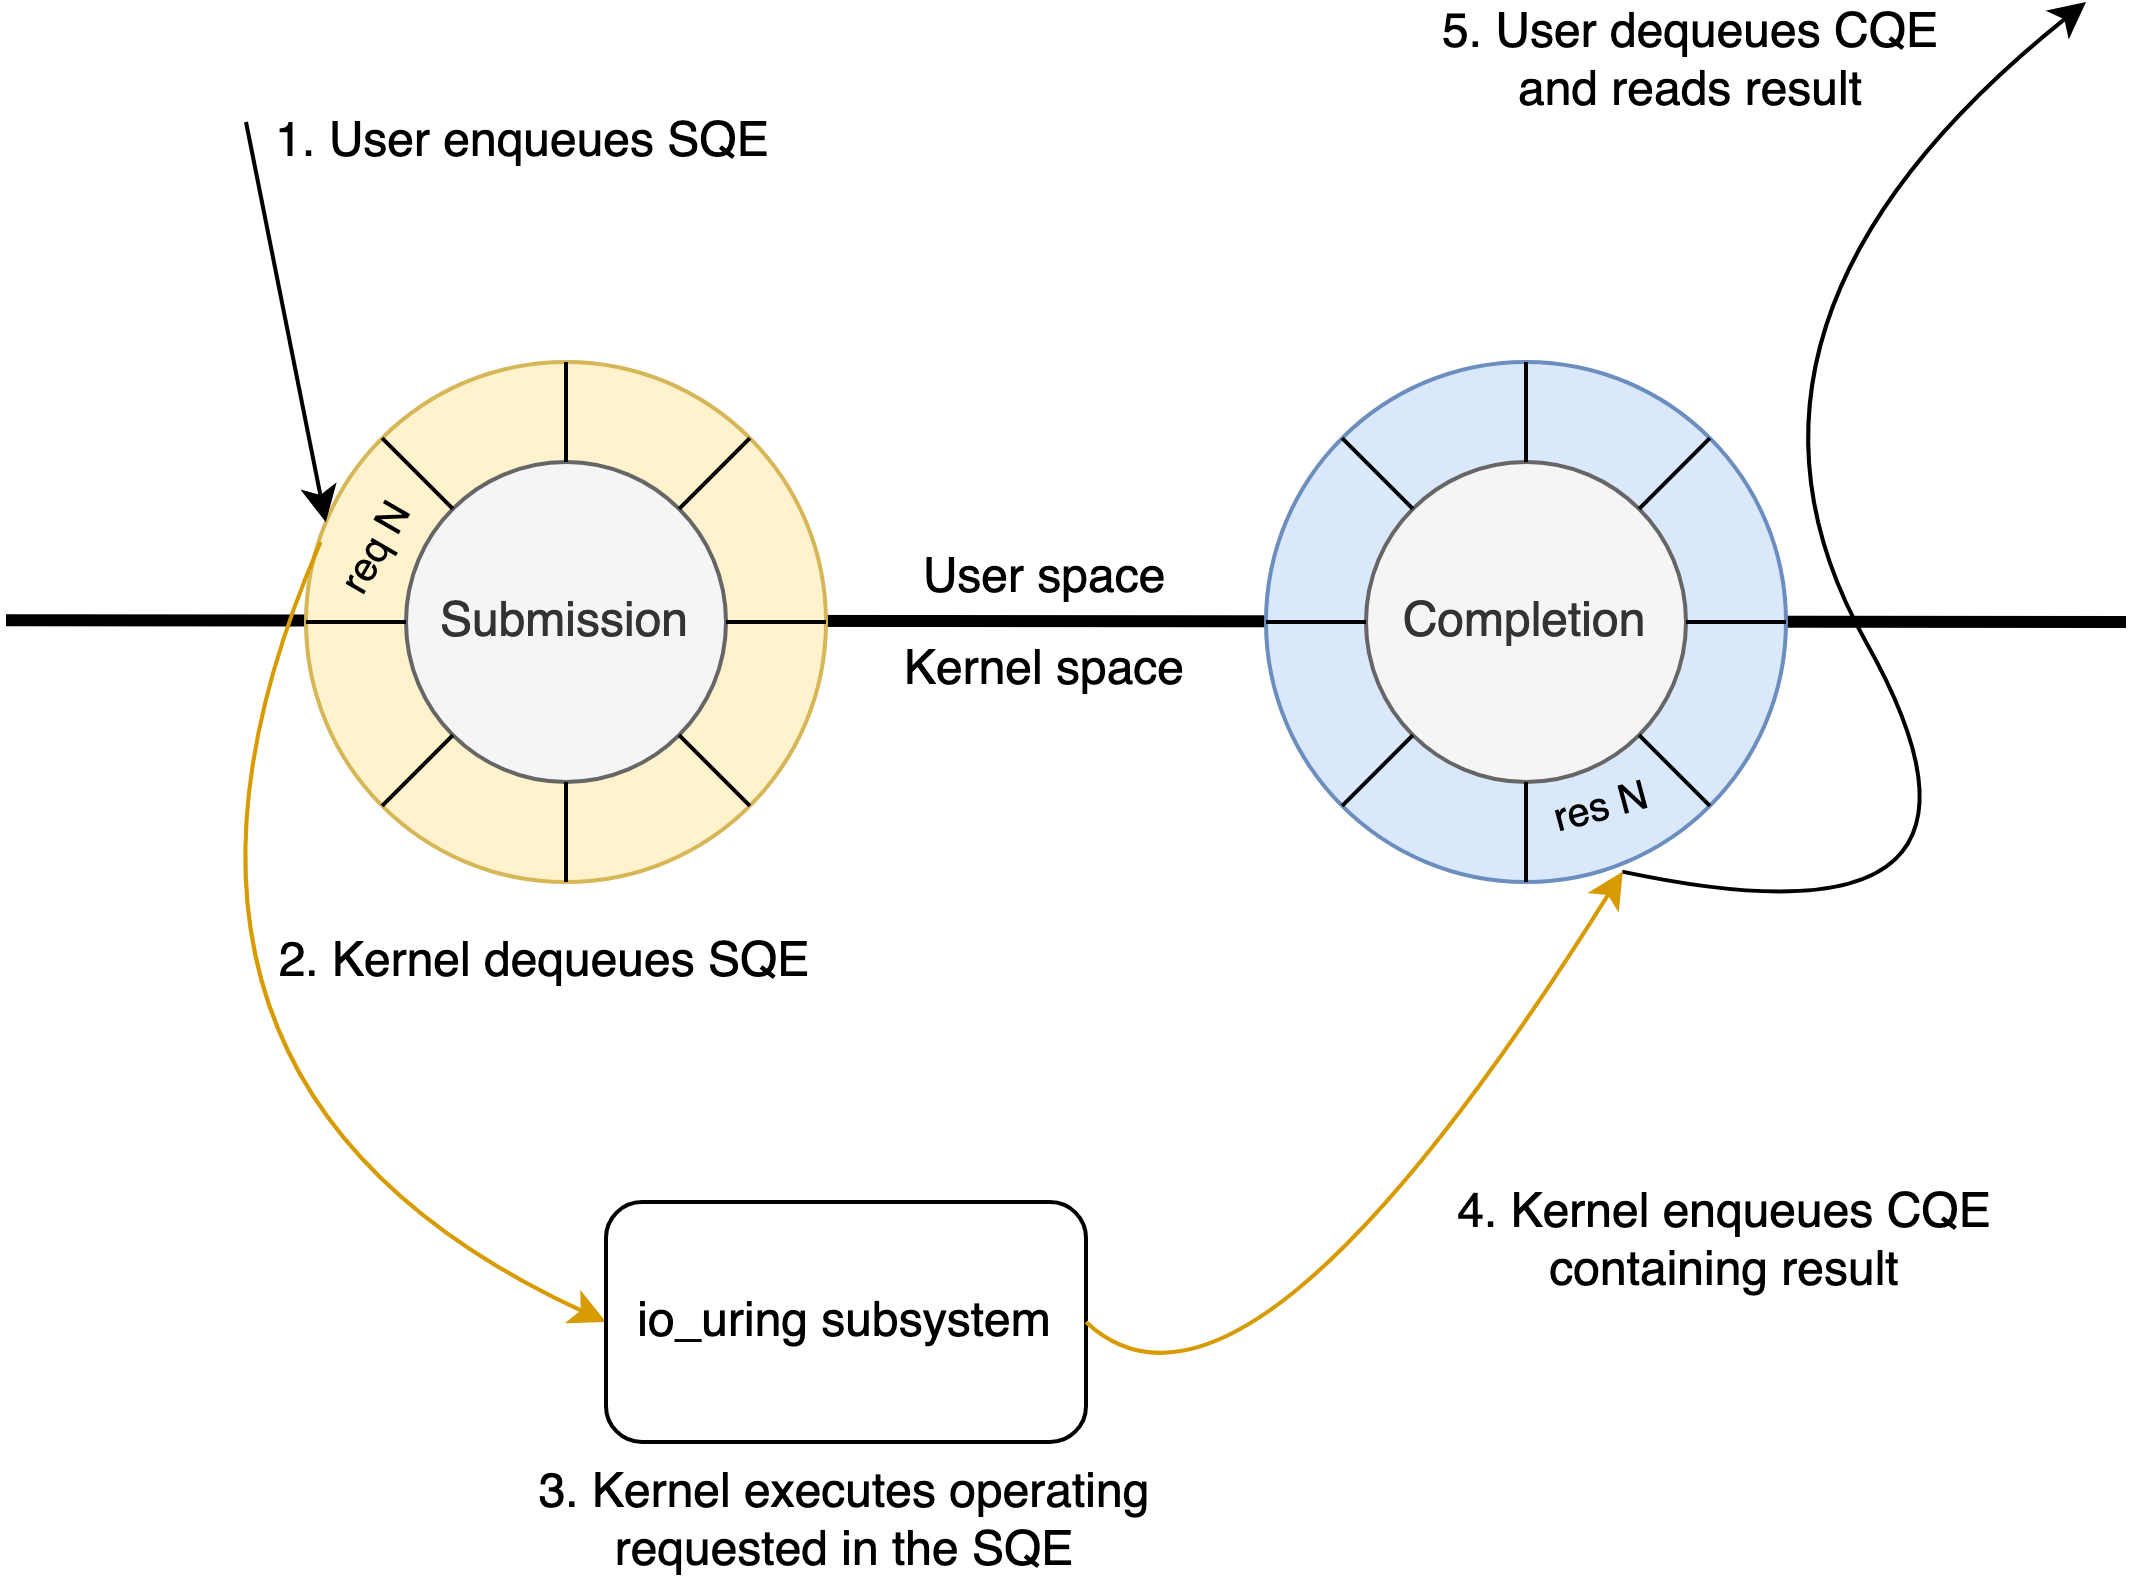
\includegraphics[width=0.85\textwidth]{figures/graphics/uring_illustrated.png}
	\caption[Usage Flow of \texttt{io\_uring}]{
      Usage Flow of \texttt{io\_uring}
	}
	\label{fig:uring_illustrated}
\end{figure} 

	\chapter{Existing Work and New Contributions}

\section{Existing Benchmarks} 
There have been mixed results in trying to demonstrate the performance benefits of the \texttt{io\_uring} interface. For networking workloads, at the time of writing, there have been a lot of open unresolved issues showing that \texttt{io\_uring} had equivalent if not worse performance compared to epoll \cite{gh_uring_issue_1,gh_uring_issue_2,gh_uring_issue_3}.

On the other hand, in the case of storage I/O, for the same workload, a specifically configured \texttt{io\_uring} was able to achieve an 80\% increase in throughput over the existing Linux Asynchronous I/O (AIO) interface, and throughput just 15\% lower than the Storage Performance Development Kit (SPDK) API \cite{understandingStorage}.


\section{Existing Work in GHC}
This paper builds off of existing unfinished work in the GHC project.
There are draft merge requests for an \texttt{EventManager} \cite{uring_event_manager}
backend based on \texttt{io\_uring}, as well as an unfinished work-in-progress
\texttt{URingManager} \cite{uring_manager_original}. Furthermore, there are aforementioned existing Haskell
bindings to \texttt{io\_uring} that both merge requests and our URingManager utilize
\cite{uring_bindings}.

An important realization made in the merge request discussion regarding
an \texttt{io\_uring} \texttt{EventManager} backend is that it would not fully take advantage
of \texttt{io\_uring}’s ability to make submit system calls asynchronously.
Since \texttt{epoll} is a system call, what the \texttt{io\_uring}-backed \texttt{EventManager}
did was use \texttt{io\_uring} to submit \texttt{epoll} requests registering
file descriptors, then keep track of requests, followed by notifying
threads upon file descriptor readiness.

\section{Our Contributions} 
We complete the unfinished \texttt{URingManager} merge request into a
working solution and iterate on our design with different performance
optimizations. Next, we modify the Haskell \texttt{network} library to use the
\texttt{URingManager} when available. Finally, we benchmark a simple Haskell
web server backed by our modified \texttt{network} against the same server
backed by the original \texttt{network} library.
	\chapter{Design Considerations}

\section{Similarities to MIO}
We noticed that an asynchronous syscall manager abstracting
over \texttt{io\_uring} had many similar design requirements to
the \texttt{EventManager}, namely:
\begin{enumerate}
	\item Allowing threads to submit requests,
	along with a post-completion callback

	\item Polling loop that checks for new events and
	executes callbacks if necessary; ready file descriptors
	in the case of the \texttt{EventManager}, completed
	system calls in the case of a hypothetical syscall manager

	\item One manager per Capability
\end{enumerate}

Hence, in our design of the \texttt{URingManager},
we draw heavy inspiration from the \texttt{EventManager}

\section{Tight Coupling with MIO \texttt{EventManager}}

The \texttt{network} library we used in our benchmarks was found
to be tightly coupled to the MIO \texttt{EventManager} and the threadWait API.
 
In Figure \ref{fig:networkThreadWait}, we depict code used to send the contents of a buffer
via a socket as of version 3.1.4.0. The \texttt{sendAll} function first attempts
to call \texttt{send}, a wrapper around a non-blocking send system call.
If unsuccessful with zero bytes sent, \texttt{threadWaitWrite} is called,
before re-attempting the send once the socket is ready. 

\begin{figure}[ht]
	\centering
	\lstinputlisting[language=Haskell]{figures/code/Network.hs}
	\caption[Sample code from the \texttt{network} library]{
		Sample code from the \texttt{network} library on Hackage
		version 3.1.4.0 demonstrating tight coupling
		to the \texttt{EventManager} \texttt{threadWait} API.
		Slight modifications were made from original source to
		improve understandability.
	}
	\label{fig:networkThreadWait}
\end{figure}
  
In order to have the network library take advantage of our \texttt{URingManager} backend,
we would have to write
completion-based counterparts of waiting-for-readiness logic.
We demonstrate this later in the \textbf{Example Usage} subsection of this current section.

Beyond the \texttt{network} library, the aforementioned discussion applies
more generally to any other code that depends on
\texttt{threadWait\{Read, Write\}}. Code written with the polling
paradigm is inherently incompatible with our \texttt{URingManager}’s completion paradigm.

This observation led us to conclude that despite the similarities in
design requirements with the \texttt{EventManager}, a completely separate design would
better suited than attempting to encompass the functionalities of
both \texttt{io\_uring} and \texttt{EventManager} in one design.

\section{\texttt{URingManager} API}

We now explain the API to \texttt{URingManager} shown in
Figure \ref{fig:uringManagerAPI}.
The main entry point into \texttt{URingManager} is the
function $\texttt{submitBlocking}$. The user passes in
a function of type $\texttt{UserData} \to \texttt{SqeBuilder ()}$
which describes what values to write into an SQE. The user needs
to have their function accept the \texttt{UserData} field
because the \texttt{user\_data} field inside
the \texttt{io\_uring\_sqe} struct is managed by \texttt{URingManager}.

Upon calling \texttt{submitBlocking}, the \texttt{URingManager}
will use the provided \newline \texttt{SqeBuilder ()} to fill in the next
free SQE, and then submit it into the submission queue of
\texttt{io\_uring}. The calling thread then goes to sleep.
Once \texttt{URingManager} receives the corresponding
result, which it keeps track of using the \texttt{UserData} field,
the calling thread gets woken and is passed on the result value.

\begin{figure}[ht]
    \centering
	\lstinputlisting[language=Haskell]{figures/code/URingAPI.hs}
	\caption[\texttt{URingManager} API]{Core \texttt{URingManager} API}
	\label{fig:uringManagerAPI}
\end{figure} 


\section{Example Usage}

In this section, we illustrate retrofitting the \texttt{sendBuf}
function in the \texttt{network} function to take advantage of
the \texttt{URingManager} when possible. This \texttt{sendBuf}
function is used under the hood of the previously
shown \texttt{sendAll} function.

In Figure \ref{fig:URingManagerExample.hs}, we add a check
to see if \texttt{URingManager} is supported. If so,
we use \texttt{submitBlocking} to submit a \texttt{send} request.
If there is no support, we fall back to the existing path
of attempting to call a non-blocking synchronous
\texttt{send} syscall and registering the socket file descriptor
to wait for write-readiness if necessary.

\begin{figure}[H]
	\centering
	\lstinputlisting[language=Haskell]{figures/code/URingManagerExample.hs}
	\caption[Example usage of \texttt{URingManager} in the \texttt{network} package]{
		Example usage of \texttt{URingManager} in the \texttt{network} package
	}
	\label{fig:URingManagerExample.hs}
\end{figure}

\section{Implementation Details} 
In our design, we use a \texttt{URingManager} data type to maintain the state of an \texttt{io\_uring} instance as well as handle incoming submissions and completions. This includes, but is not limited to, references to the \texttt{io\_uring} file descriptor itself, the submission and completion queue, an \texttt{IntMap} dictionary keeping track of in-flight \texttt{io\_uring} submissions, and a unique number generator. The definition of URingManager is shown in Figure \ref{fig:URingManager}.

\begin{figure}[ht]
    \centering
	\lstinputlisting[language=Haskell]{figures/code/URingManager.hs}
	\caption[\texttt{URingManager} Definition]{\texttt{URingManager} Definition}
	\label{fig:URingManager}
\end{figure} 



In particular, the \texttt{requests :: IntMap} is a table mapping from a unique UUID to callback. For each SQE, we generate a unique number using the generator inside the URingManager, and write that value to the \texttt{user\_data} field of the SQE. Upon receiving the CQE corresponding to the SQE, using the \texttt{user\_data} field in the CQE, we look up the `requests` mapping to find the corresponding callback to perform.


\begin{figure}[ht]
    \centering
	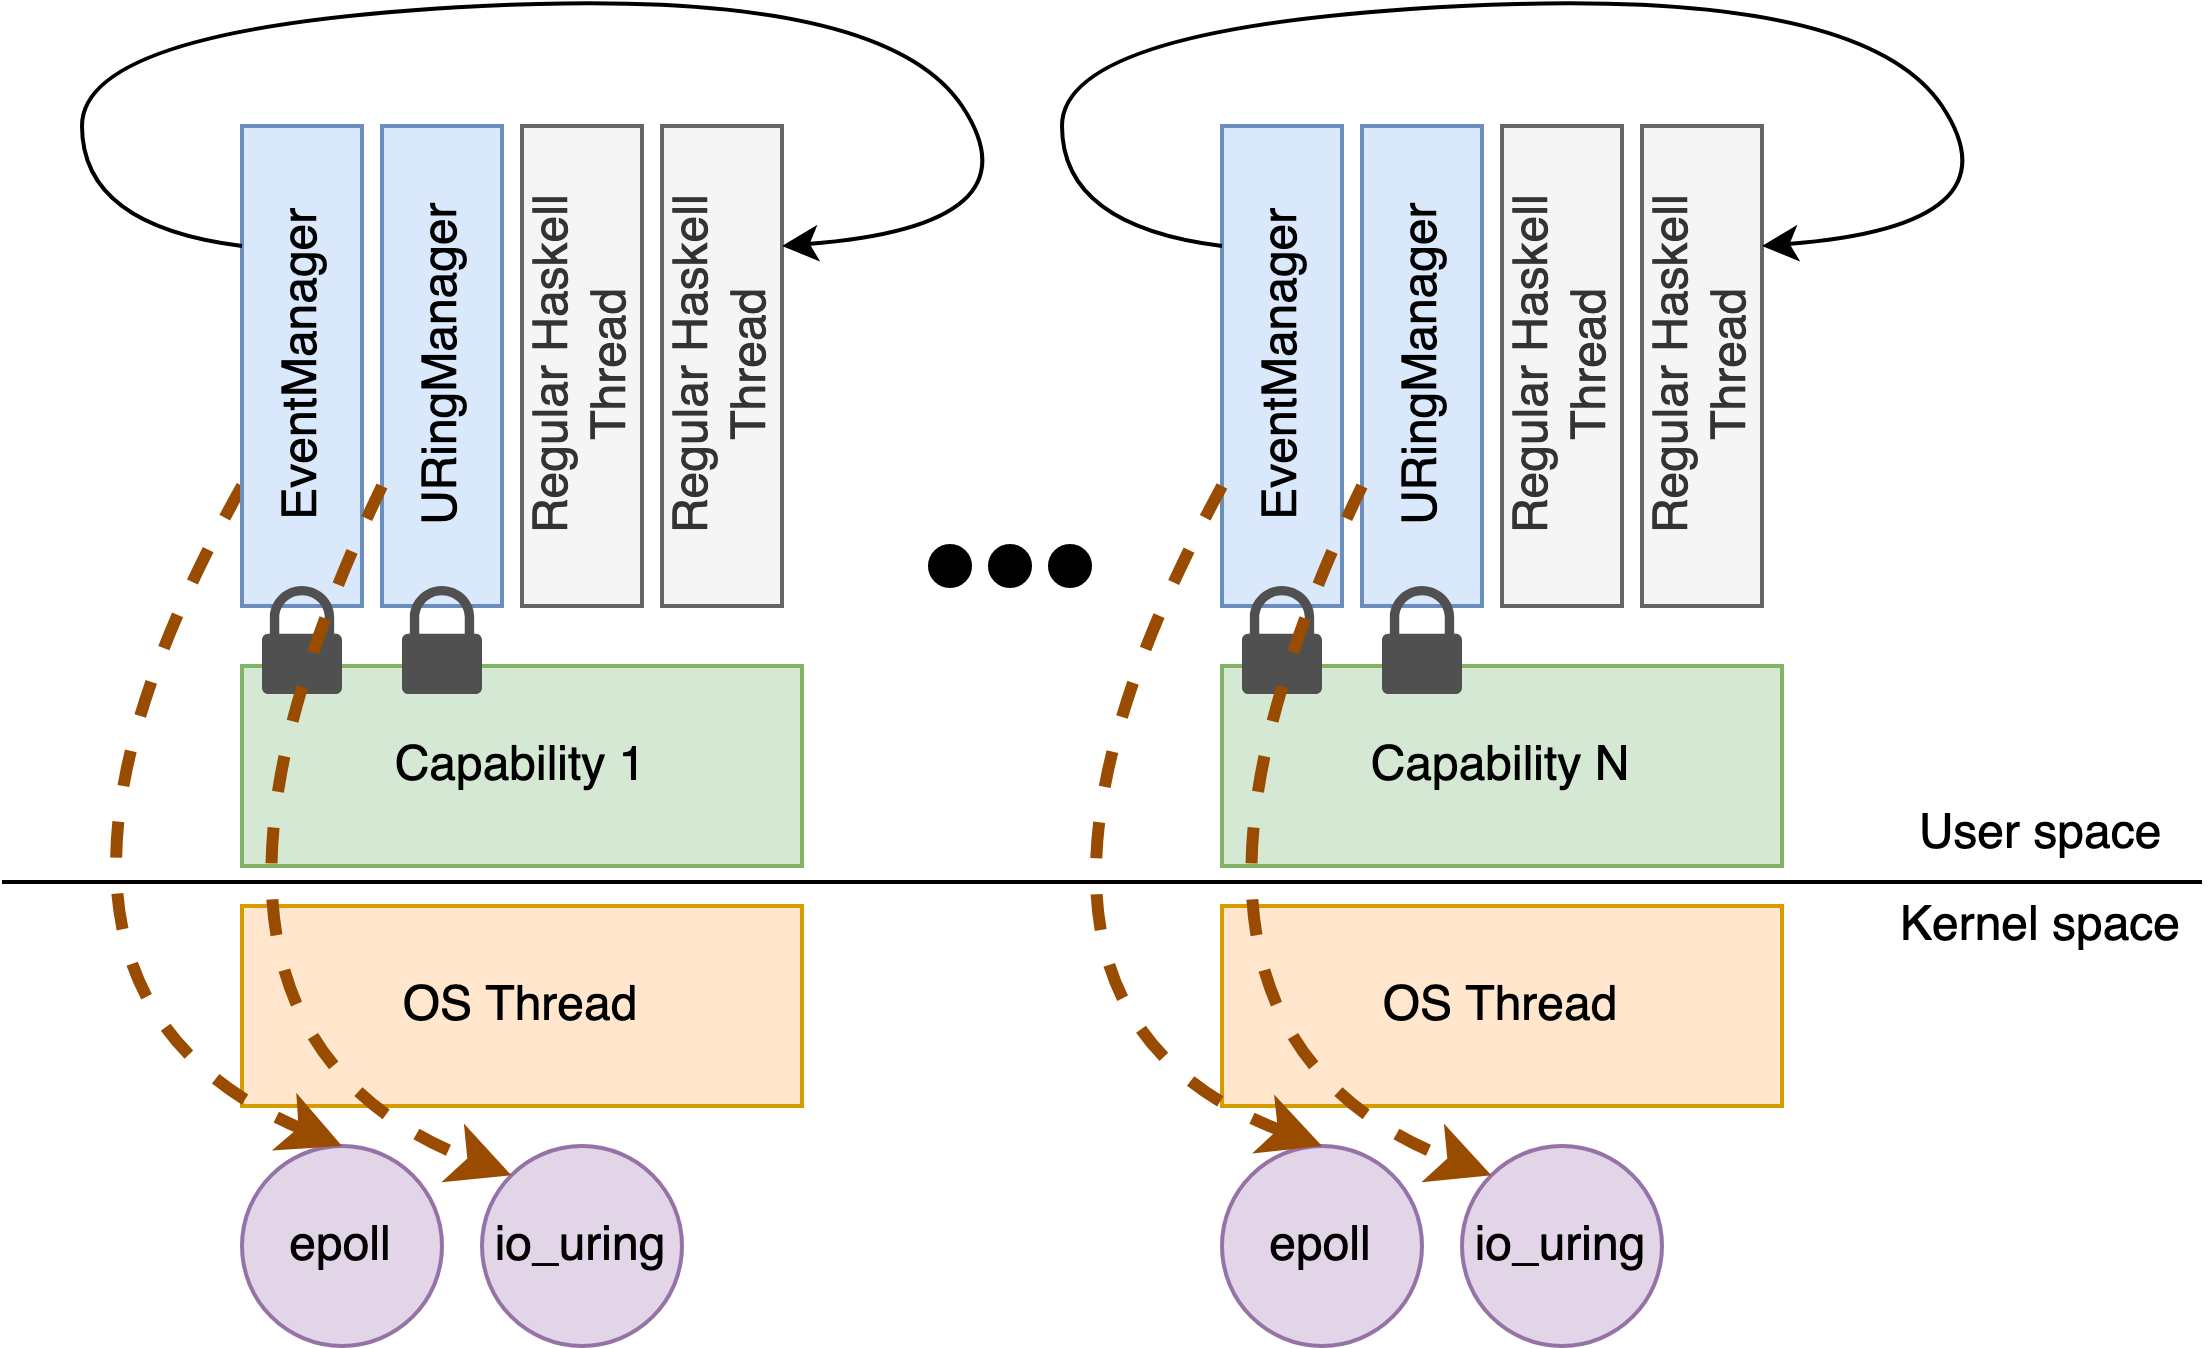
\includegraphics[width=0.85\textwidth]{figures/graphics/ghc_illustrated.png}
	\caption[Big Picture: Capability, \texttt{URingManager}, and \texttt{EventManager}]{
		Illustration of how Capabilities, \texttt{URingManager}, and \texttt{EventManager}
		fit in together in the GHC RTS.
	}
	\label{fig:ghc_illustrated}
\end{figure} 


For each Capability, we create a corresponding Capability-local \texttt{URingManager} value, and spawn a corresponding Capability-bound thread that polls for and handles new completions in a loop. Thus, the number of \texttt{io\_uring} file descriptors open is equal to the number of Capabilities set by the user. Associating each Capability with a \texttt{URingManager} and polling loop was directly inspired by each Capability having an \texttt{EventManager} and polling loop too. Refer to Figure \ref{fig:ghc_illustrated} for an illustration of how the Capability, \texttt{URingManager}, and \texttt{EventManager} fit into the GHC RTS. 


\section{Other Potential Approaches}

We alternatively considered the approach of extending the \texttt{EventManager} to become an asynchronous system call facility. In this scenario, we would extend the \texttt{EventManager} interface to include asynchronous system calls such as read and write. Registering a file descriptor can be seen as another supported system call. For the existing polling-based \texttt{EventManager} backends, implementing the asynchronous write syscall for example would involve first registering the file descriptor for writes, and then actually executing the write system call when the file descriptor is known to not block.

There were two main potential benefits from such a design. Firstly, a generalized \texttt{EventManager} would be less ad-hoc than having a separate \texttt{URingManager} interface that libraries have to conditionally depend on if the operating system is a recent-enough version of Linux. Secondly, although not tested, the \texttt{URingManager} would have to run in an additional Haskell thread, meaning potentially larger overhead.

Nevertheless, we ultimately decided against this unifying design for the following reasons. It would be hard for the unifying design to cover all possible implementation-specific requirements that other programs may have. Furthermore, it would have a higher maintenance burden for RTS maintainers to cover the addition of new system calls and implementation changes over all operating systems. Finally, the additional Haskell thread is not a concern as these threads are lightweight, and it is possible to disable either the \texttt{EventManager} or \texttt{URingManager} threads in the program if not used.

	\chapter{Optimizations}
\section{Kernel Polling Mode} 
Instead of submitting the \texttt{io\_uring\_enter} system call to notify the kernel
of new entries, we can use a kernel thread to continuously check the submission
queue for new entries. To enable this is as simple as enabling the
\texttt{IORING\_SETUP\_SQPOLL} on setup.
Again, this is in the \texttt{io\_uring} theme of reducing syscalls.

\section{Multi-shot SQEs}

In general, each SQE being submitted corresponds to a single CQE received.
However, in newer kernel versions, multi-shot SQEs have been introduced.
As opposed to the existing one-shot SQEs, multi-shot SQEs can return multiple CQEs when applicable.
For instance, the \texttt{accept()} system call is used to assign the next new connection to a new socket file descriptor.
In the case of both the regular synchronous \texttt{accept()} and
the \texttt{io\_uring} \texttt{IORING\_OP\_ACCEPT} asynchronous request,
upon exiting and receiving each new connection, another accept syscall has to be made again to accept the next connection.
With the multishot variant of \texttt{IORING\_OP\_ACCEPT},
the kernel will continuously queue up new CQEs containing connection results without
the user process having to rearm the submission queue with another accept request.
This is more efficient because in the non-kernel polling case, this saves an
\texttt{io\_uring\_enter} syscall, and in either case, saves the kernel from having to process an additional SQE.

To implement support for multi-shot SQEs, we modify the requests table
inside the \texttt{URingManager} to keep track of whether a request is multi-shot or one-shot. 
Additionally, instead of deleting the entry upon receiving a CQE corresponding to a
multi-shot SQE, we simply keep it in the requests table. Last but not least,
for multi-shot SQE submissions, rather
than a callback that does \texttt{putMVar}, we store a callback that spawns a new Haskell
thread bounded to the same Capability (via \texttt{forkOn} because the direct file table
is local to that specific Capability) that handles the results instead.

% STRETCH GOAL
% Figure X shows the pertinent code changes.

\section{Fixed File Descriptors}

At the kernel level,  in multi-threaded contexts, sharing a file descriptor table has a non-trivial overhead.
A recent new development in \texttt{io\_uring} allows the usage of thread-local file descriptors and file descriptor tables, in what is referred to as fixed file descriptors.
Fixed file descriptors have the same semantics as regular file descriptors, except they are managed by a user-allocated local file descriptor table.
Therefore, these local fixed file descriptors are only valid in the same thread.
These fixed file descriptors are operated on what is referred to as direct variants of existing syscalls/wrapper functions.
For example, in liburing, there is both an \texttt{io\_uring\_prep\_accept()} and an \texttt{io\_uring\_prep\_accept\_direct()} wrapper function.

Furthermore, it is also possible to pre-assign fixed file descriptors
to syscall requests, such as \texttt{open()}-ing a file at a specific fixed file descriptor.
However, we do not take advantage of this pre-assigning ability in our \texttt{URingManager} design.

In order to accommodate fixed file descriptors in our \texttt{URingManager}, we most significantly had to change
the way we scheduled our Haskell lightweight threads.
In our original design, it was possible for a Haskell thread to submit an SQE to different
\texttt{URingManager}s and therefore \texttt{io\_uring} submission queues between different requests.
This is possible because the \texttt{URingManager} interface only allows for submitting the SQE request
to the \texttt{URingManager} corresponding to the Capability that is currently executing the submitting Haskell thread,
and Haskell threads are not necessarily bound to a specific Capability.
The solution is to make sure that Haskell threads using fixed file descriptors in their
logic need to be spawned with \texttt{forkOn} in order to be tied to a Capability.


% TODO: STRETCH GOAL
% Compare Figure Y to Figure Z to see the corresponding differences in code in order to
% support fixed file descriptors and multi-shot SQEs.

	\chapter{Benchmarking}
\section{Web Server Benchmark Program}
We slightly modify the simple HTTP web server program
used to benchmark MIO \cite{mio} for own benchmark.
We use our version of the \texttt{network} library that supports our URingManager. The web server, listening on a specified address, receives HTTP requests and then responds with a fixed HTTP response regardless of received content.

When benchmarking, we test two versions of the server: one without URingManager (using default \texttt{epoll EventManager}) and one with \texttt{URingManager}. We initially wished to benchmark a modified version of our \texttt{URingManager} with all the mentioned optimizations in the previous section, however, our implementation unfortunately would frequently hang. This made it impossible to reliably test. 
The main parts of the server are shown in Figure \ref{fig:WebServer}

\begin{figure}[ht]
    \centering
	\lstinputlisting[language=Haskell]{figures/code/WebServer.hs}
	\caption[Benchmarked Web Server Source]{Main parts of our web server}
	\label{fig:WebServer}
\end{figure} 

The sources are all included in the monorepo \url{https://github.com/zyklotomic/uring-manager}.

\section{Setup} 
We used Apache Bench (\texttt{ab}) to measure the time taken for 10,000  default HTTP requests of size 151 bytes each with a variable number of concurrent connections to be processed by our web server.

Hardware-wise, an AMD Ryzen 5 2600 Six-Core Processor with 16 GB of RAM was used. The Linux kernel version used was 6.4.3 on the NixOS distribution.

Both the Apache Bench and the web-server program were running on the same CPU. In order to minimize variance caused by scheduling, the Linux \texttt{cpuset} mechanism was used to reserve 8 cores for the web-server program only, and 1 core for the single-threaded Apache Bench. Kernel threads were allowed to run on the aforementioned reserved cores.


	\chapter{Results}

\begin{figure}[ht]
    \centering
	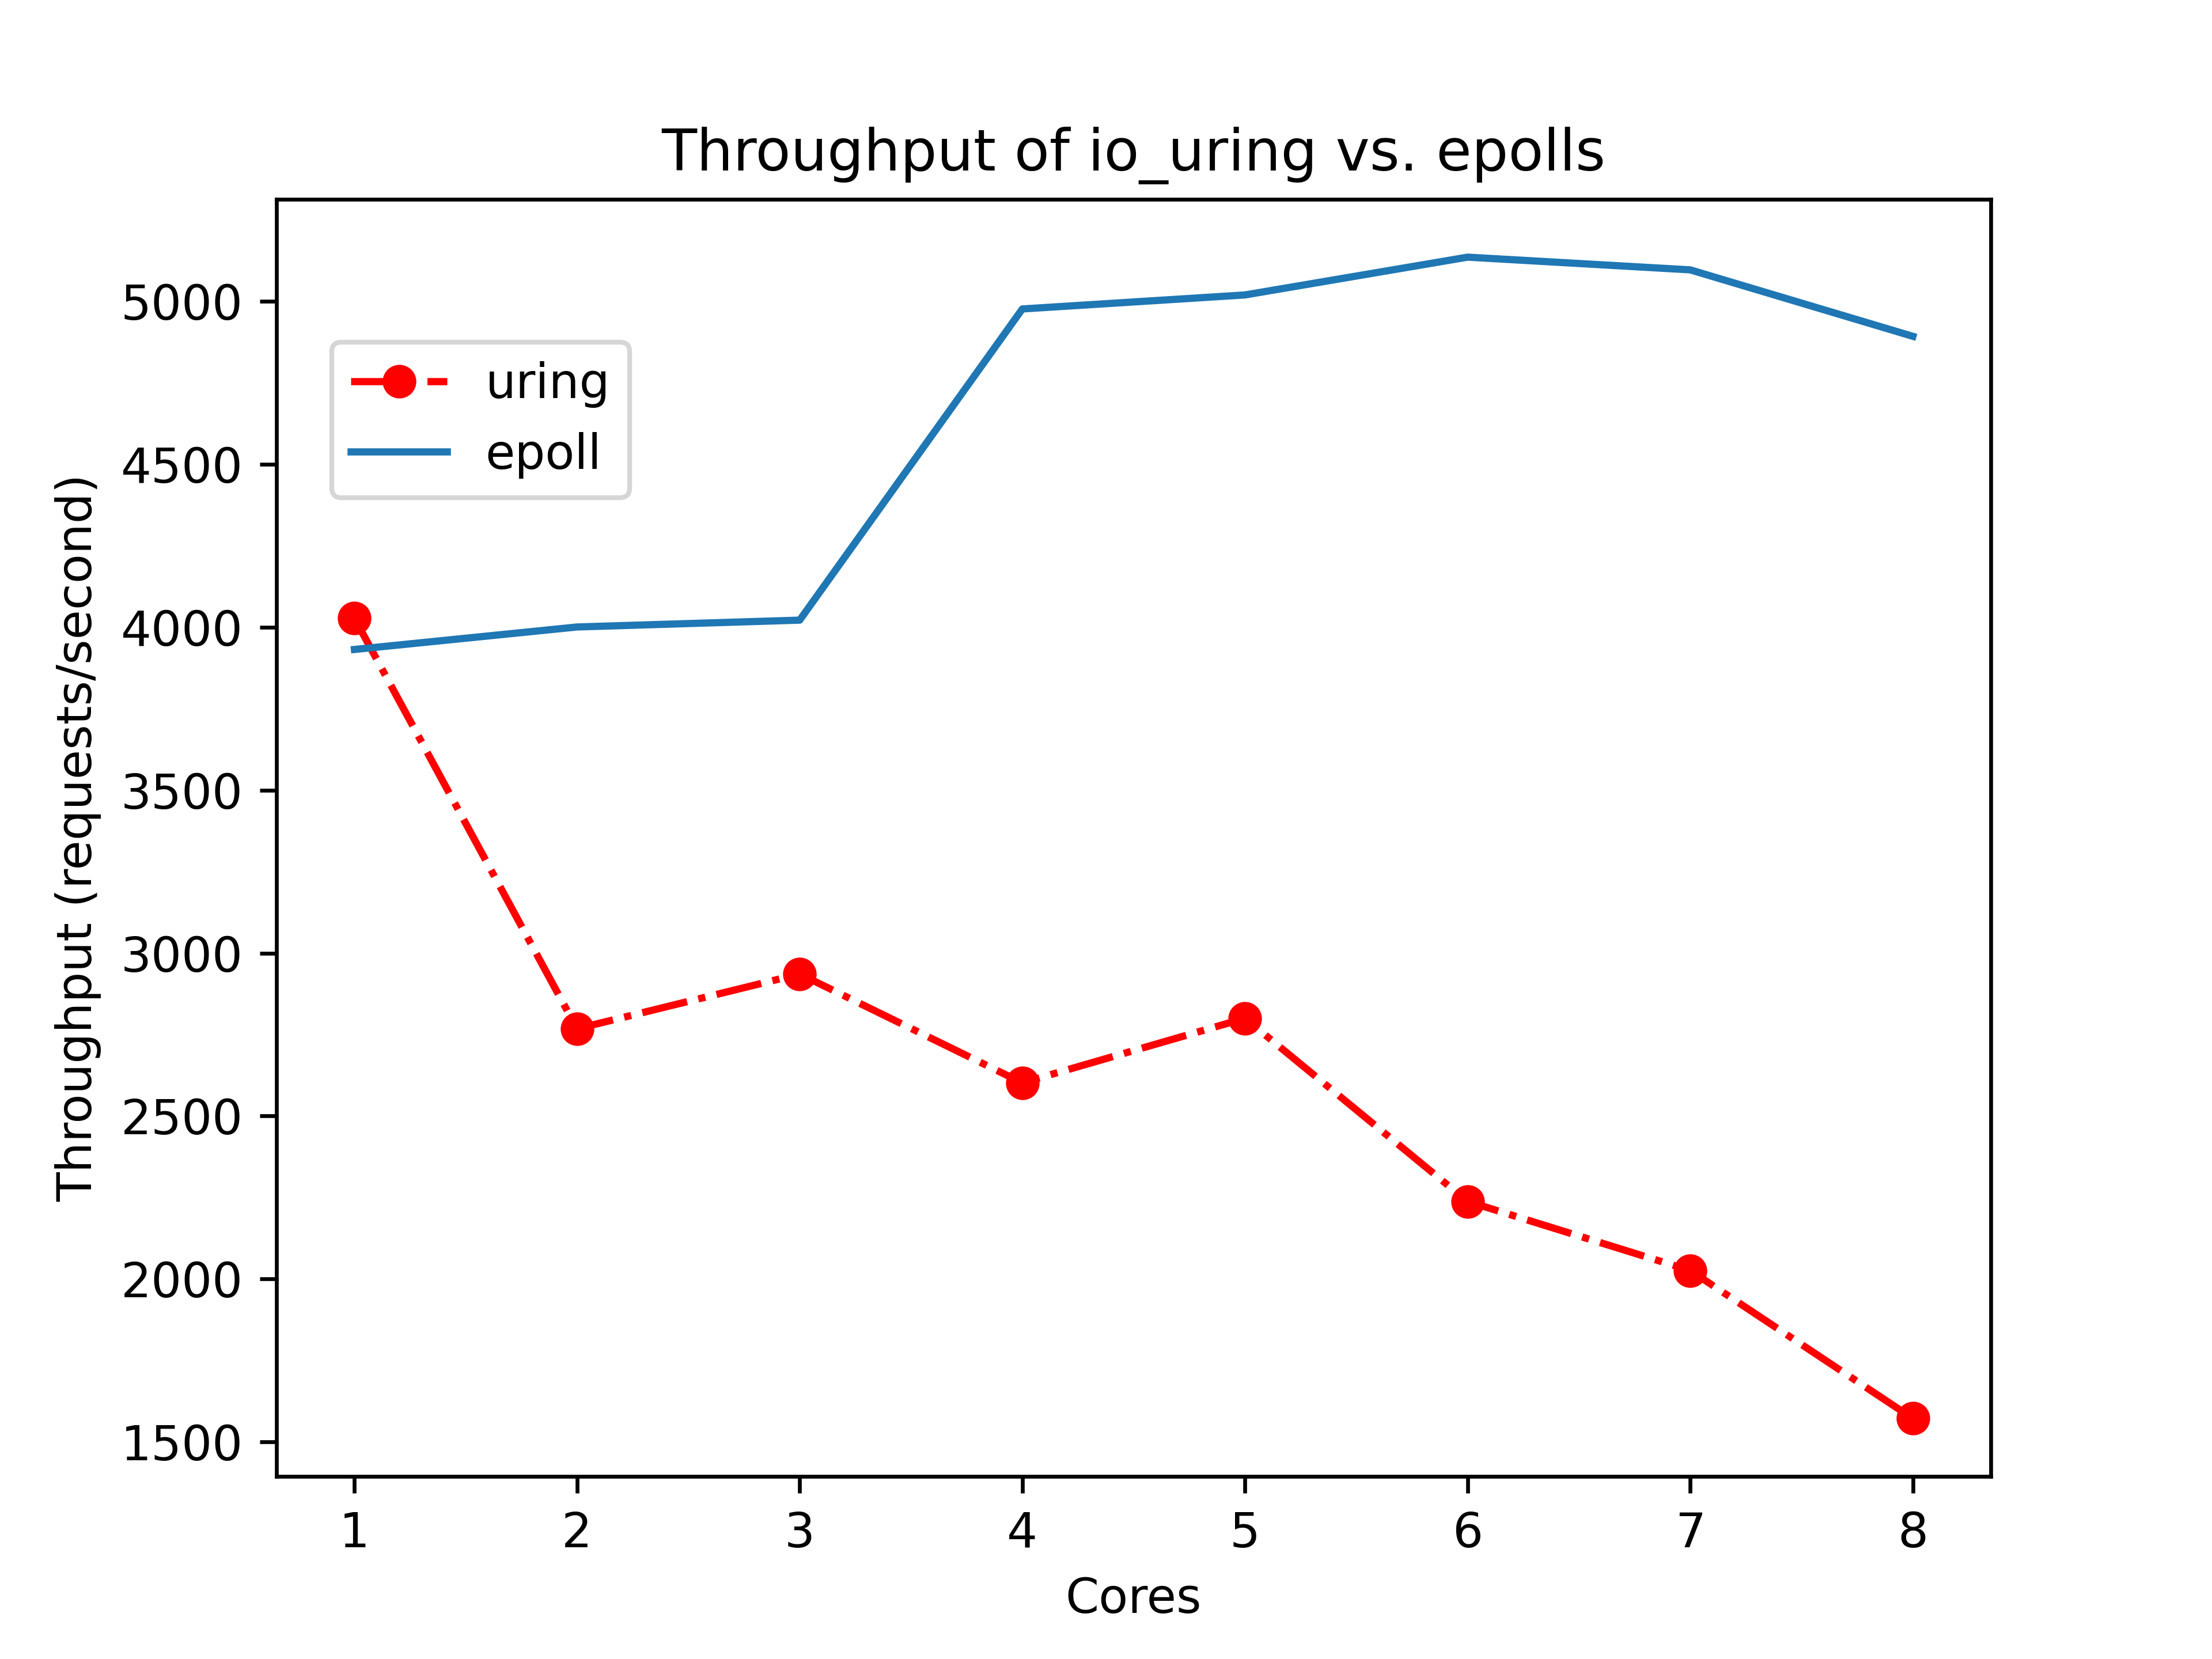
\includegraphics[width=0.85\textwidth]{figures/graphics/throughput.png}
	\caption[Web Server Throughput]{
		Graph comparing the throughput of the \texttt{io\_uring URingManager} web server
		and the \texttt{epoll EventManager} web server. Benchmarked by sending
		10,000 requests and 50 concurrent connections
	}
	\label{fig:throughput}
\end{figure}

For this section, we will refer to the \texttt{io\_uring} case interchangeably as the \texttt{URingManager} case, and likewise for epoll being interchangeable with \texttt{EventManager}.

In the single-Capability case, with 50 concurrent connections, and \texttt{URingManager} at 4028 kilobytes per second vs. \texttt{EventManager} at 3923 kilobytes per second, \texttt{io\_uring} has a very negligible lead in throughput over epoll. However, \texttt{io\_uring} performance worsens as the Capability count increases. As for \texttt{EventManager}, throughput increases slightly as Capability count increases up until it plateaus at around 6 Capabilities. These observations
regarding throughput can be seen from Figure \ref{fig:throughput}. 

\begin{figure}[ht]
    \centering
	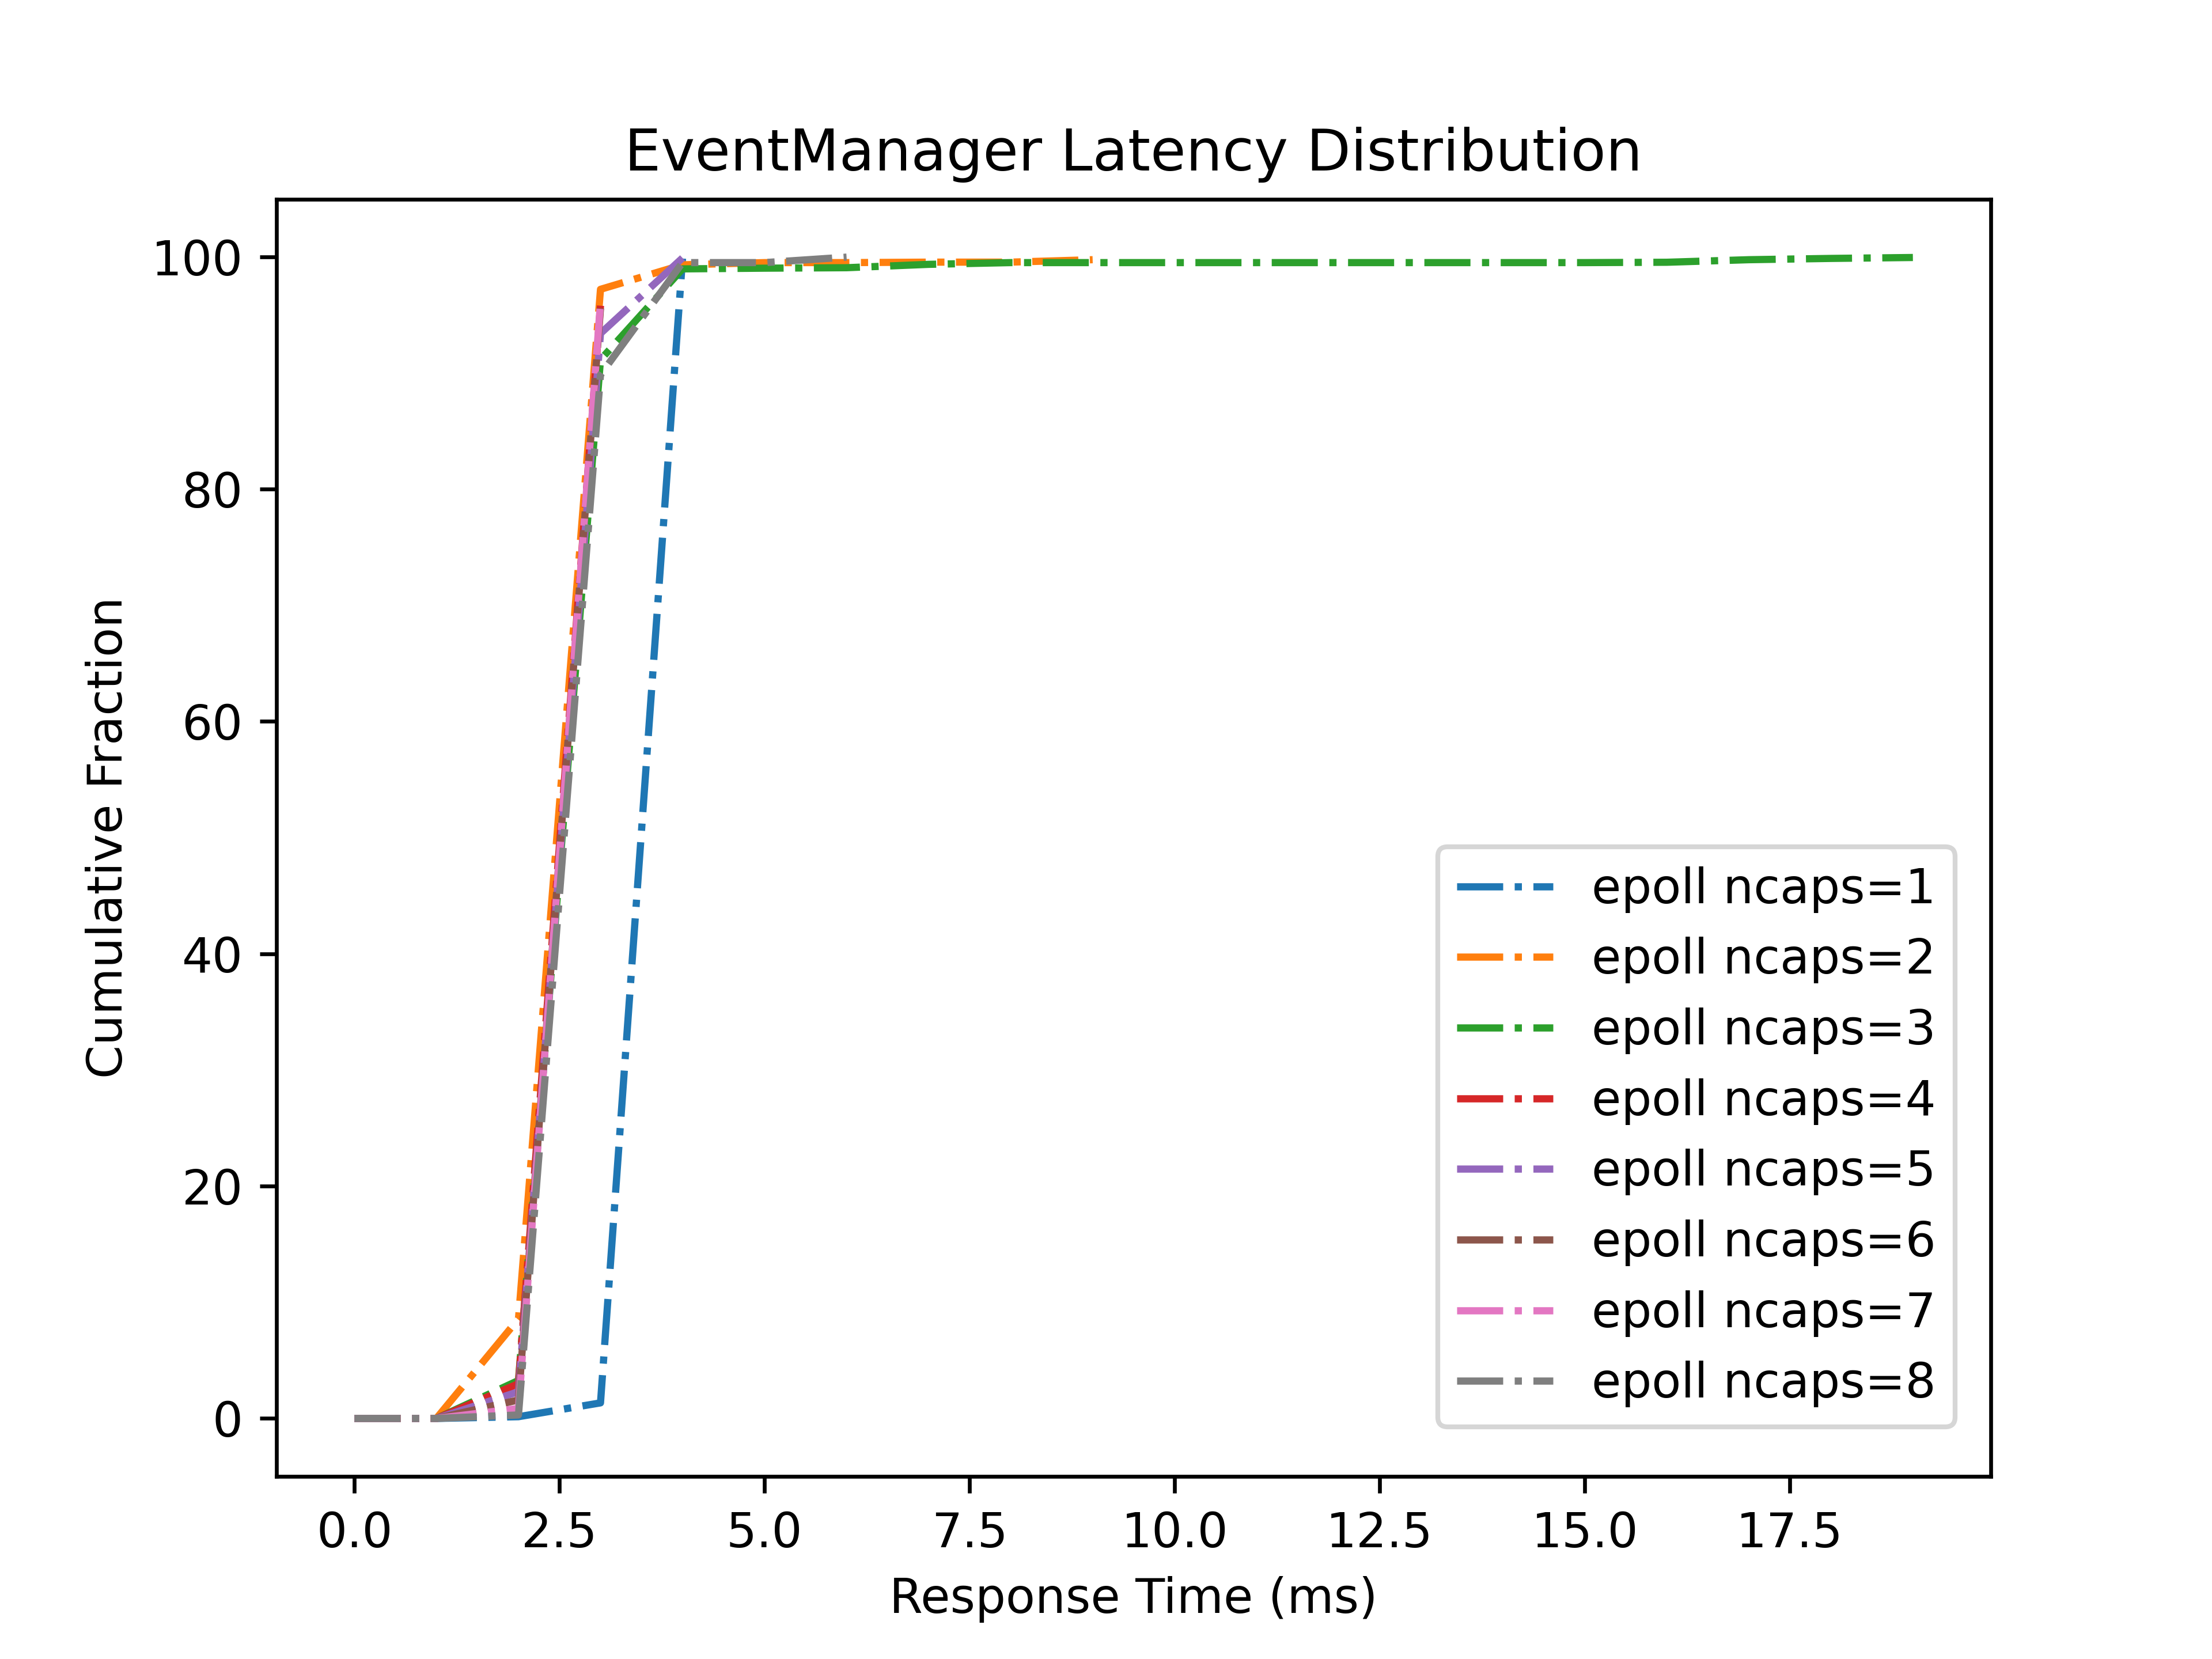
\includegraphics[width=0.85\textwidth]{figures/graphics/epoll_latency.png}
	\caption[\texttt{epoll EventManager} Web Server Latency]{
		Cumulative Distribution of latencies of the \texttt{epoll EventManager} web server
		program over 10,000 requests and 50 concurrent connections
	}
	\label{fig:epoll_latency}
\end{figure}

\begin{figure}[ht]
    \centering
	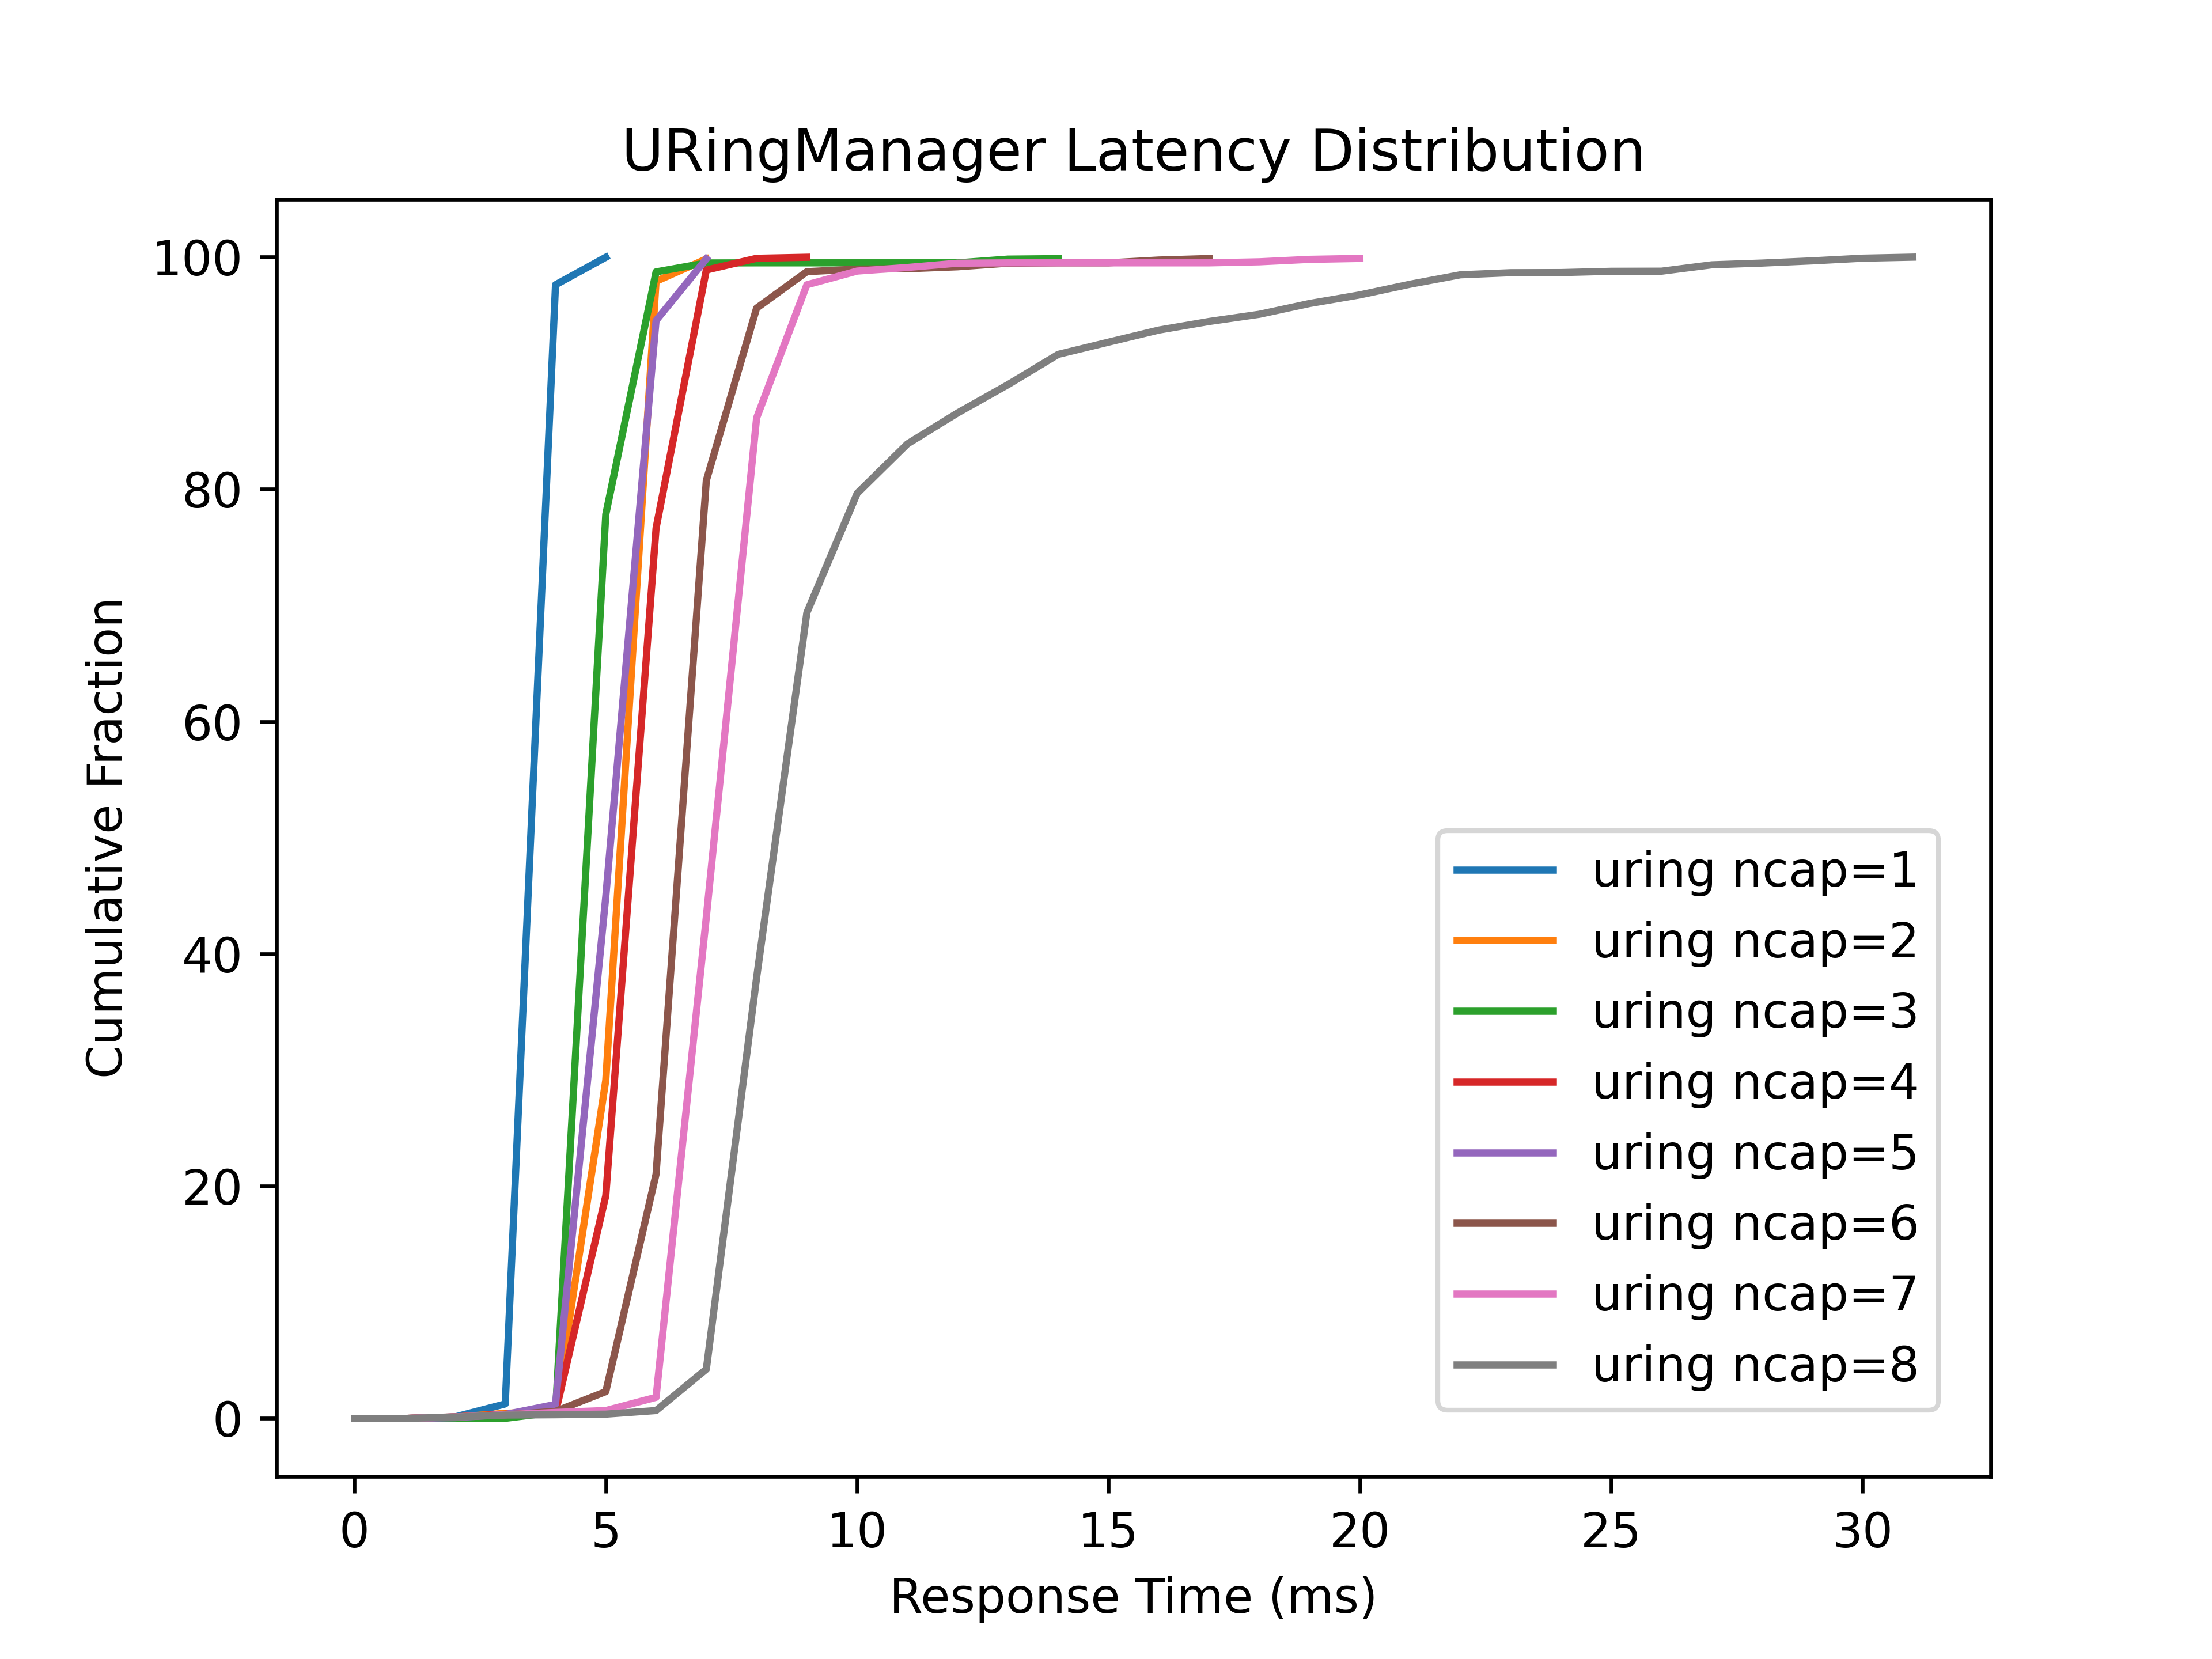
\includegraphics[width=0.85\textwidth]{figures/graphics/uring_latency.png}
	\caption[\texttt{io\_uring URingManager} Web Server Latency]{
		Cumulative Distribution of latencies of the \texttt{io\_uring URingManager} web server
		program over 10,000 requests and 50 concurrent connections
	}
	\label{fig:uring_latency}
\end{figure} 


As for tail latency, the single core \texttt{io\_uring} case is comparable to
\texttt{epoll} as shown in the Cumulative Fraction graphs.
Like with throughput, tail latency is worse as the number of URingManager capabilities increase;
compare Figure \ref{fig:epoll_latency} and \ref{fig:uring_latency}.
	\chapter{Discussion}
\section{Analysis of Results} 
From our benchmarks, we conclude that in the single-core case, \texttt{URingManager} is on par with \texttt{EventManager} in a networking workload. As for scaling, \texttt{URingManager} does not scale with the number of Capabilities. Throughput is actually inversely proportional to the number of Capabilities for \texttt{URingManager}, with progressively worse throughput the higher the number of Capabilities.

We also observe that our results for the \texttt{EventManager} are in line with the findings in the paper that introduced the MIO \texttt{EventManager}; specifically, that throughput scales linearly with the number of Capabilities. The plateauing around 6 Capabilities is to be expected since the benchmarks were run on a 6-core processor.

The  \texttt{io\_uring} \texttt{URingManager} also had significantly worse latencies for the higher percentiles of response time for high Capability counts. This would have made sense in the case of batched SQE submissions, where we submit and notify the kernel of new SQEs in batches, and thereby trading individual latency for throughput. However, we did not use submission batching in our \texttt{URingManager}. An alternative reason is that from a user space program, how the kernel processes and schedules new SQE submissions is a black box, and the internal kernel logic optimizes for overall throughput over individual latency.

\section{Potential Setup Issues}
The setup used to conduct the experiment was not optimal because there is a chance that both our web server that we benchmark and Apache Bench, the benchmarking program, were running on the same computer. Despite the usage of \texttt{cpuset}, the web server may have been bottlenecked by the CPU having to simultaneously schedule Apache Bench as well, having to accommodate the extra reads and writes of Apache Bench.

Ideally, both programs would be running on two separate computers with a 10 Gigabit or above direct connection so as to remove all bottle-necks not pertaining to the web-server itself.

\section{Design Merits of \texttt{io\_uring} and \texttt{URingManager}}
Besides performance, \texttt{io\_uring} also aimed to be a cleaner replacement interface for asynchronous system calls over the existing Linux Asynchronous I/O (AIO) interface. AIO was notorious for being difficult to use and inconsistent.

Issues of AIO include no support for buffered I/O, support for only direct file I/O, lack of glibc bindings, and that the API does not guarantee non-blocking calls.
% (https://man7.org/linux/man-pages/man2/io_submit.2.html).
Regarding the last point on blocking calls with AIO, it can happen for example if the programmer inadvertently passes in a file descriptor backed by a filesystem without non-blocking support into AIO’s \texttt{io\_submit} syscall. In short, it is hard to reason about whether an operation is truly non-blocking with AIO. \texttt{io\_uring} completely solves this problem because its design is fundamentally asynchronous. Even if a file descriptor does not support non-blocking, submitting an SQE is definitely a non-blocking operation.

% http://blog.vmsplice.net/2015/08/asynchronous-file-io-on-linux-plus-ca.html


Thus, despite its performance shortcomings in this paper, the design and usage experience of \texttt{io\_uring} is appreciated. We feel that this clean design trickles down into the design of URingManager too. Instead of interfacing with the EventManage to register interest and then perform the actual desired request, Haskell programmers can simply submit a request to URingManager. The completion-paradigm helps simplify the model of asynchronous computation.

% https://lwn.net/Articles/776703/

	\chapter{Future Work}

\section{More Rigorous Benchmarking} 
As mentioned under our Discussion section, the benchmarking ideally would have been run on a multi-computer rather than a single-computer setup. With an optimal benchmarking setup, we can be more certain of the reason behind why our \texttt{URingManager} did not perform as good as our theoretical expectations for \texttt{io\_uring}. Furthermore, we were only focused on network I/O workloads. It would be worthwhile to benchmark file I/O with the \texttt{URingManager} too.

\section{Optimizing \texttt{URingManager}}
The \texttt{epoll} interface was introduced in Linux kernel version 2.5.44, in 2002,
which was over two decades ago. Meanwhile, \texttt{io\_uring} was first introduced in kernel 5.1 in May 2019. Unlike \texttt{io\_uring}, we have had many years to perfect how to use epoll to achieve its full potential. The theoretical reasoning of \texttt{io\_uring} using less system calls and therefore more performant is there, we believe that we just have not figured out the best design for using \texttt{io\_uring}. Thus, it would be  productive to further research on how to optimize the performance of \texttt{URingManager}.

\section{Vulnerabilities in \texttt{io\_uring}} 
Recently, Google’s security team stated in a report of their vulnerability bounty program that 60\% of submitted exploits involved \texttt{io\_uring}. As a result, Google has disabled \texttt{io\_uring} in a few of their Linux-based products such as Android and ChromeOS, as well as in their production servers \cite{google_security}. Due to the infancy of \texttt{io\_uring}, the alarming number of vulnerabilities is not unexpected. Nonetheless, \texttt{URingManager}, and any other usage of \texttt{io\_uring} is not mature enough for production usage until further work is done to ensure the safety of exposing the \texttt{io\_uring} interface. Possible research directions could include formal verification as well as more vulnerability bounties.

\section{Windows I/O Completion Ports} 
Windows has I/O Completion Ports (IOCP), a very close equivalent to \texttt{io\_uring}. Similar to \texttt{io\_uring}, IOCP also features a queue to submit requests such as reading and writing to files, and sending to and receiving from sockets. It would be of interest to explore making a unified I/O queueing interface as a generalized \texttt{URingManager} so that we can support IOCP as well.

\section{Generalization of the Event Manager}
Building on generalizing \texttt{URingManager} for Windows IOCP, an alternative approach is generalizing
EventManager to manage all types of asynchronous requests, of which \texttt{URingManager} is one
implementation. While we did decide against this approach as mentioned in our Design Considerations,
we believe this idea is still worth exploring. We can implement a generalized EventManager for \texttt{epoll}
by having the manager under the hood handle both registering file descriptors to epoll in addition to
the actual requested system call. The benefits of such a generalized EventManager would be a more
unified interface and more portable Haskell code. However, the major downsides would be the
increased maintenance burden in the GHC RTS and the potential inflexibility if a more custom request scheduling policy is desired.

    \makeBibliography
\end{thesisbody}

\end{document}
